\documentclass[11pt]{article}
\usepackage{amsmath}
\usepackage{graphicx}
\usepackage{longtable}
\usepackage{color}
\usepackage{tabu} %% text tables
%%\usepackage[linktocpage=true]{hyperref} %% links to numbers instead of sections
\usepackage{hyperref}
%%\usepackage{url}
\usepackage{geometry}
\geometry{left=3.5cm,right=3.5cm,top=3.5cm,bottom=3.5cm}
\graphicspath{{./WP_images/}}
\usepackage{amsmath}
%%\usepackage{cite} 
%%\usepackage{notoccite}
\usepackage[backend=bibtex,sorting=none]{biblatex}
\addbibresource{wp-refs.bib}




\begin{document}



\title{%
Lifestyle Exchange Token (LYF)\\Decentralized Experience Exchange (DXEX)\\[1mm] 
\large Blockchain Based Lifestyle Exchange}
\author{Bluvato Inc.}
\date{\today}
\maketitle


\begin{abstract}
People acquire assets in order to add value to their lives, from a pair of golf clubs, to a motorboat, to a classic 1969 Camaro. These are not the types of items or experiences that people want to expend the time or energy to market/rent, nor do they want to entirely sell these assets. Currently, the only viable option is all or nothing -- hang on to your assets and enjoy them on occassion, or sell them and lose all their benefit. Lifestyle Coin (LYF) and the Decentralized Experience Exchange (DXEX) unlock the potential for people to exchange experiences with each other, but retain their original assets and fiat currency. LYF and DXEX allow for the creation of new value in assets that previously had no practical earning potential, while unlocking new opportunities of exchange for rich lifestyle experiences. Additionally, DXEX allows for the connection of consumers and sellers of luxury items that were previously inaccessible or unknown. DXEX utilizes a token-based sytem to allow for trades between unrelated parties and assets. Consider the following exampe: You want to find someone who wants to borrow your jet ski in Miami, in exchange for the use of their Ferrari in San Diego. Practically, it would be impossible for you to set up this kind of trade. Instead, the LYF token serves as a unit of intermediary value, where the value of LYF is pegged to its attractiveness in the community compared to other experiences. LYF fuels the marketplace for individuals to exchange lifestyle events. DXEX allows for a decentralized exchange of high-value, low liquidity assets, unlocking liquidity and utility in previously underused assets.

\end{abstract}
\pagebreak

\tableofcontents
\newpage

\section{Value Proposition}
\label{sec-2}

We propose the \textrm{LYF} as a token of exchange in order to provide a secure, liquid currency to trade these non-liquid assets and experiences. The \textrm{LYF} system provides: 
\begin{itemize}
\item{Membership: membership into an exclusive, global club of like-minded individuals who want to consume and share world-class experiences. }
\item{New Opportunities: even among friends, there is not an incentive to assume the risk of trading a coveted asset without anything in return. Human beings are rational creatures, and seek a return on their lending, particularly if they are assuming risk of loss or damage. LYF provides this return by allowing these users to consumes other experiences. }
\item{Security: with the entirety of these lifestyle exhanges on the Ethereum Blockchain, there will not be a so-called "trusted" third-party who can impose unnecessarily high transaction fees or favor certain parties. The entire history of both the payment, exchange, and reviews of these experiences will persist in perpuity within a decentralized ledger, accessible by all.}
\end{itemize}
\section{The Challenge}
\label{sec-3}

\begin{quote}
\textit{``Share your toys.''}
\end{quote}
We are taught from a young age that we should share our toys. Fast forward a few years and we pass on this same wisdom to our children. Realistically, we do not practice what we preach.

Outside a very narrow range of family and perhaps close friends, we do very little to meaningfully share our adult toys. As as adults our toys usually correspond to assets like properties, vehicles, domiciles or other items that in some way contribute to a more interesting life "experience."

The few times we share as adults is usually among friends and family. We are self-interested people. Currently there is no platform for us to meaningfully lend our items or those things comprising an experience and to expect a trade in turn that eclipses the risk associated with lending our things out. 
\section{Decentralized Experience Exchange and Life Exchange Token}
\label{sec-4}

To create a new platform and unity of exchange for illiquid, but valuable experience.

The first component involves the roll-out of a new exchange, DXEX -- Decentralized Experience Exchange -- and a community portal that will allow users to post rich media/text descriptions about about the details and veracity of their items and exchanges.

The Exchange itself does not need to be a fully polished product, at first. Instead, like Craigslist, it can be a relatively simple--but incredibly powerful--exchange that allows for the posting of information. 

The LYF is the token for the Decentralized Experience Exchange.

\begin{center}
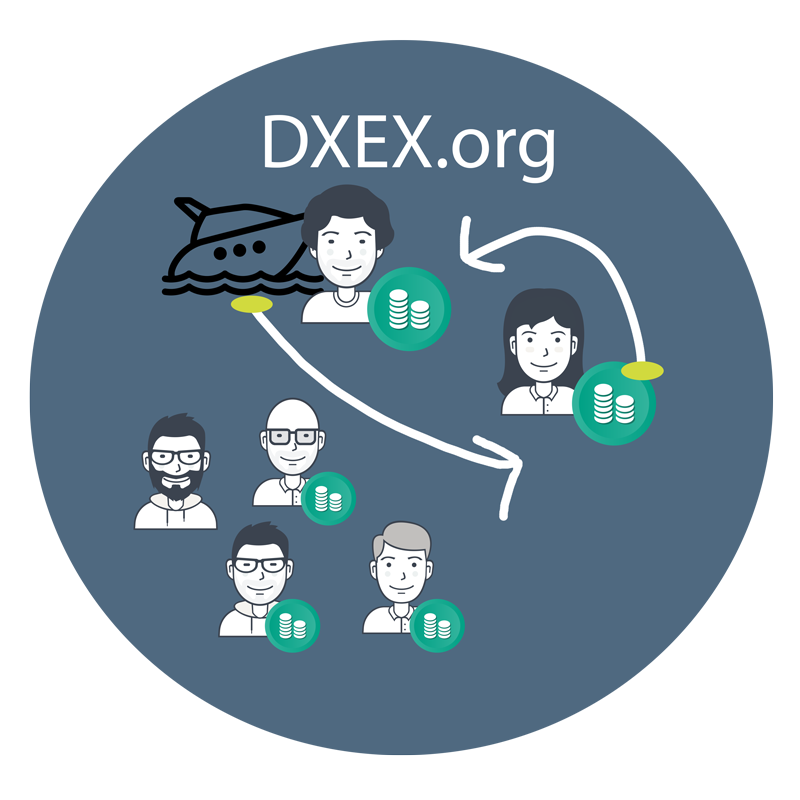
\includegraphics[width=.8\textwidth]{dex1.png}
\end{center}

Why the LYF is more efficient and useful than fiat currency is because it unlocks a new paradigm for exchange. It does not make sense to rent your goods for fiat currency / fiat money, because then you are effectively competing with an entire industry, in fact, two industries -- the hospitality industry and the entertainment industry.

By not allowing for users to deal in fiat currency, this creates a more egalitarian and exclusive club in order to allow people to exchange goods for goods -- experiences for experiences. This is a labor of love, not profit.

The exchange itself does not expressly discourage the use of the platform in order to profit. Although highly respected and enjoyable members of the community can and will sit on stockpiles of the token, the token itself will--long-term--only be of value if it can unlock interesting and unique experiences. In the area of market speculation for the tokens an a third-party exhange, the act of market speculation could and potentially would drive the price to unreasonable heights/lows, but this is not the primary focus of the token. An explosition of interest in a price move tied to the LYF could offer a short-term interest in the exchange itself, providing much needed publicity needed for the exchange to succeed.

Additionally, a reasonable amount of third-party speculation can be helpful for the efficiency of the marketplace, allowing for increased liquidity for those who want the LYF token. However, sustained market speculation will only serve to devalue the application of the exchange, thereby decreasing the relative value of the tokens. So-called "market makers" or "whales" would be well served to only provide enough liquidity so that the overall marketplace can still enjoy the fruits of the exchange, lets they find that their pernicious hoarding/market manipulation devalues the efficiency of the exchange, and therefore devaluing the tokens themselves.

Additionally, DXEX has another safeguard against the ill effects of market speculation. Because the DXEX should only have value in exchanging experiences, if the LYF token itself is way overvalued/undervalued, the market itself can correct by the individuals adjusting their prices accordingly to reach closer to an equilibrium. If you wanted to rent a Ferrari for 100 LYF, you should want to do so at 120. To make up the 20-point gap, you are incentivized to list more experiences on the exchange. As the exchange reaches critical mass and increasingly liquidity assets are exchanged, then the ability of any one market manipulator is lessened by the daily average volume of transferred LYF. 

\section{Further Considerations}
\label{sec-5}

\subsection{Safety}
\label{sec-5-1}
The safety of the platform is of paramount importance to both the short-term and long-term objectives of the Decentralized Experience Exchange. In order to achieve this goal, the platform will incorporate the following:
\begin{itemize}
\item{Blockchain ledger: the transaction, bid, communication, reviews, and other ancillary information will be stored in the public ledger}
\item{Profiles and pictures: similar to social media platforms such as Facebook, club members will be encouraged to post pictures of themselves in order to build a sense of community and transparency. }
\item{Third-party identify management and identification tools: these will be optional, but likely highly useful in serving to regulate the community.}
\item{Common sense: as with other platforms like Craigslist, those users who write clear, convincing experiences, and provide useful pictures and/or videos in order to allow someone to evaluate the experience will be rewarded with more eyeballs and repeat customers. All things equal, experiences that do not pass the smell test--no verified reviews, no pictures, and scant details--should be reasonably ruled out by potentially interested third-parties by applying the smell test.}
\item{Forum: a forum can be used to identify common risks, scams, and scammers. Similar to the way that CL uses "flags" to review users and/or posts, these kinds of scammers and/or scams will be identified and regularly reviewed by the community. If needed, more sophisticated tools, captchas, and/or a decentralized approval process for creation of new user account can be adopted by the community.}
\item{Voting: significant changes/improvements to the website design will take be put to a vote, and only users who have been a part of verified experience exchanges will be given a vote. The voting mechanism should be engaged on the blockchain by allowing those users with an experience to have a vote. All votes will be equal regardless of amount of LYF held or number of transactions completed. }
\end{itemize}

\subsection{Community}
\label{sec-5-2}
There will only be value in the Decentralized Experience Exchange if it successful in bringing about interesting, engaged people who want to share interesting, engaging experiences with one another. The goal of this exchange is not to make money or profit from 

Because of the high transactional cost of traditional luxury items and experiences, the average person is at a disadvantage in terms of acquiring these types of rich experiences. Luxury items are not treated as commodities, and the luxury marketplace does not need to compete on price with the same fervor as commmodity markets. Rather, these luxury marketplaces compete on quality and service, with price being a tertiary concern or even not a concern at all.

\begin{quote}
\textit{
Disruption -- the good kind.
}
\end{quote}


Of course, this is not to assume that the luxury marketplace is at risk of disruption--in a negative way, at least. By exposing larger groups of people of various economic statuses to experiences that would have previously been inaccessible, this could serve to increase the expose the luxury marketplace to new buyers. The luxury vendors are not losing the customers of those people who could have never afforded their products anyway. And those people who are lucky enough to able to afford a new experience are more likely do so outright.


\subsection{Derivatives}
\label{sec-5-3}
Of course, it is entirely possible that individuals will want to take an experience for which they themselves have not earned an equivalent amount of LYF tokens to afford now. The exchange does not discourage the use of loans and derivative products -- bonds, insurance, lending pools -- so long as they provide liquidity/efficiency to the marketplace. The Ethereum platform allows for the useful and relatively easy building of such loans directly on the blockchain, and this itself could be a quite interesting and healthy application of the technology. Again, so long as these loans and derivative applications do not serve to decrease the efficiency of the overall exchange, they are a welcome and supported value-adding activities to allow more individuals to have interesting and productive experiences.

\subsection{Insurance}
\label{sec-5-4}
The topic of insurance will definitely be an important one for the community. Rather than something to be feared, this is something to be embraced by people. By using the value-adding LYF tokens in exchange for other experiences, members can offset the cost of their insurance policies. Members should due their own diligence and share their experiences in ensuring their items *prior* to posting them on the exchange. While the exchange does not want to be overly prescriptive, this is something that is a requirement to ensure the value of most high-worth experiences. If needed, the community can enact a verification to ensure that sellers post experiences only after covering them with insurance policies.

\section{Roll-Out Planning}
\label{sec-6}
How do intend to get to a fully functioning exchange? Iteratively, of course.

\subsection{Token Sale}
\label{sec-6-1}
The initial sale of the token will seek to raise at least (10) million USD at whatever the current exchange rate for ETH :: USD.

\subsection{Use of Funds}
\label{sec-6-2}
We will use the funds in order to develop the DXEX and to pursue targeted marketing/advertising activities toward driving awareness and user adoption.

Please understand that purchase of the LYF token, per say, does not imbue any ownership in the workings of the exchange, nor does it confer voting rights. Instead, LYF are to be used as the token of exchange for world class experiences.

The bulk of the funds will be used for the payment of application development and security analysis. After a working alpha is available, early adopters will have the ability to become some of the first members to use the platform. The reason for this is deualfold -- those who are early adopters and willing to invest in the platform deserve early access, and those who are willing to invest likely see value in this platform in order to exchange experiences.

\subsection{Release Planning}
\label{sec-6-3}
Here are the high-level targets for the release of the DXEX:

\begin{itemize}
\item{October 10, 2017 : \bf \underline{Token sale}}
\item{February 2018 : Release of Alpha}
\item{April 2018 : \bf \underline{Release of First Beta}}
\item{June 2018 : 2nd Beta Release}
\item{October 2018 : Application Conference}
\item{January 1 2019 : \bf \underline{Production Release}}

\end{itemize}

\section{Board of Directors and Contact}
\label{sec-7-1}

\begin{center}

\includegraphics[width=0.2\textwidth]{will.jpg}
\end{center}

\begin{itemize}
\item{Will Ulmer, Founder

\textit{An innovator, Will's diverse experience from the entertainment industry to the higher education start-up vertical to cloud application development offers him a unique and broad perspective on disruptive technologies. Apart from enterprise cloud applications developing solution consulting projects across federal, state, and non-profit sectors, Will is an investor and innovator in blockchain technologies that straddle the line between fin-tech and social good.}}
\end{itemize}

\begin{center}
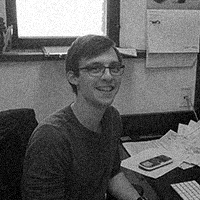
\includegraphics[width=0.2\textwidth]{anthony.jpg}
\end{center}

\begin{itemize}
\item{Anthony Veltri, Advisor

\textit{Anthony is a molecular biophysics doctoral student at Johns Hopkins University. His scientific research pertains to characterizing the crosstalk between mRNA decay and translation regulation in eukaryotes.}
}
\end{itemize}

\begin{itemize}
\item{Olalekan Lekuche, Head of International Development

\textit{Olalekan possesses a Medical degree from Olabisi Onabanjo University, a Master’s Degree from the University of Maryland, and an MBA from Johns Hopkins University. Ola possess several years of experience working as a clinician in Nigeria and on innovative projects across the healthcare industry in the United States. He was involved in the implementation of the new care delivery model helping improve outcomes and lower costs for the Centers for Medicare \& Medicaid Services, which insures over 100 million Americans.}
}
\end{itemize}



You can get in touch with the development team behind the Decentralized Experience Exchange and LYF token by reaching out to contact@getlyf.com. If you are interested in a strategic partnership with the platform, please reach out to contact@bluvato.com

\section{Attributions}
\label{sec-8-1}

\begin{itemize}
\item{User Avatars by UserInsights is licensed under CC BY 3.0,
https://usersinsights.com/}
\item{Car Avatar by http://www.adianteapps.com/}

\end{itemize}
%link: https://www.iconfinder.com/iconsets/user-avatars-1

%Need to remove boat icon : https://www.iconfinder.com/icons/172634/yacht_icon#size=128
%Coin icon : https://www.iconfinder.com/icons/1886510/bank_banking_business_coins_finance_marketing_icon#size=128
%boat : https://www.iconfinder.com/icons/1076712/boat_cruise_ocean_sea_ship_travelling_water_icon#size=128
%car : https://www.iconfinder.com/icons/339936/car_dealer_mechanic_vehicle_icon#size=128


\printbibliography

\vspace*{\fill}

\begin{flushright}
{\textcircled{c}} Bluvato Inc. 2017


% \pdfcreationdate
\end{flushright}
\end{document}
